\documentclass[margin=5mm]{standalone}
\usepackage[T1]{fontenc}
\usepackage[utf8]{inputenc}
\usepackage{pgf,tikz, pgfplots}
\usetikzlibrary{calc}
\usetikzlibrary{intersections}
\pgfplotsset{compat=newest}
\usetikzlibrary{shapes}

\begin{document}

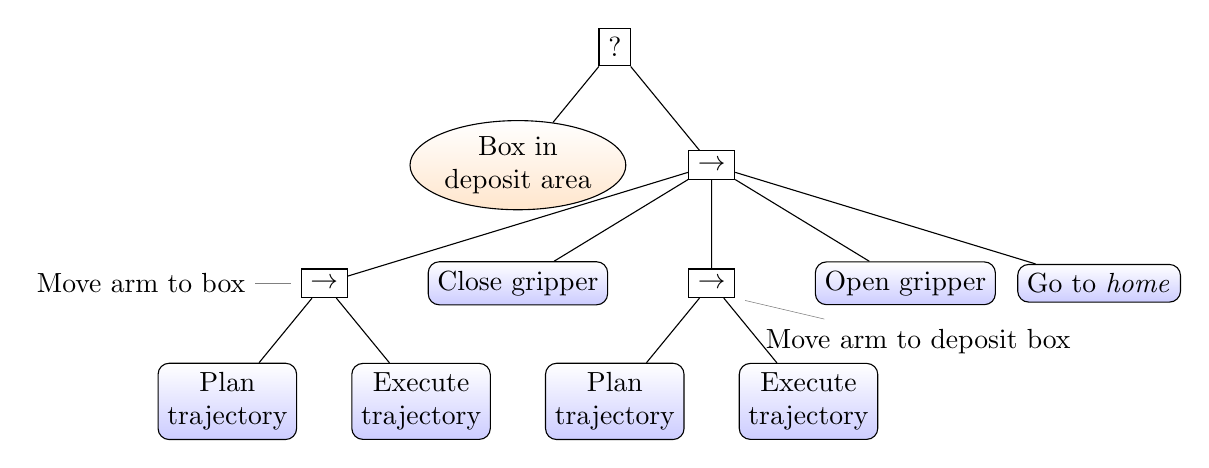
\begin{tikzpicture}[sibling distance=7em,
  condition/.style = {shape=ellipse, draw, align=center,
    top color=white, bottom color=orange!20, inner sep=1pt},
  sequence/.style = {shape=rectangle, draw,},
  fallback/.style = {shape=rectangle, draw,},
  action/.style = {shape=rectangle, rounded corners,
    draw, align=center,
    top color=white, bottom color=blue!20}]]
  \node[fallback] {?}
  child { node[condition] {Box in\\deposit area} }
  child { node[sequence] {$\rightarrow$}
    child { node[sequence, ] (tobox) {$\rightarrow$}
      child { node[action] {Plan\\ trajectory} }
      child { node[action] {Execute\\ trajectory} }
    }
    child { node[action] {Close gripper} }
    child { node[sequence, ] (todeposit) {$\rightarrow$}
      child { node[action] {Plan\\ trajectory} }
      child { node[action] {Execute\\ trajectory} }
    }
    child { node[action] {Open gripper} }
    child { node[action] {Go to \emph{home}} }
  };

  \node[pin=180:{Move arm to box}] at (tobox.west) {};
  \node[pin={[pin distance=2mm] -45:{Move arm to deposit box}}] at (todeposit.south east) {};
  
\end{tikzpicture}

\end{document}
